\section{Initial Theory}
In terms of a Wireless Channel, it is preferred for the receiver to be able to estimate the state of the wireless channel. This can allow for optimisations to be made for optimal propagation of signals from transmitter to receiver. For the receiver to understand the state of the wireless channel, many models exist which explain the properties and state of the channel.
\subsection{WLAN Channel Model}
%%%%%%%%%%%%%%%%%%%%%%%%%%%%%%%%%%%%%%%%%%%%%%%%%%%%%%%%%%%%%%%%%%%%%
A wireless channel model describes how the amplitude and phase of a signal change as it propagates from the transmitter to the receiver. Of particular importance to this project is the propagation model of a channel. The main propagation models are large-scale propagation known as large-scale path loss and small-scale propagation known as small-scale fading \citep{articleWLAN}. Doppler spread can also be considered. \par
Large-scale path loss describes the attenuation of a signal between the transmitter and receiver due to physical phenomena in the environment. As the physical environment constrains the wireless signals, the received signals convey information about the environment that they pass through. It is clear that as the distance between transmitter and receiver is increased, the signal and thus, signal power, is spread over a larger area suffering greater attenuation. Small scale fading occurs due to the scattering environment caused by obstacles between the transmitter and receiver changing with time \citep{articleWLAN}. Transmitted signals arrive at the receiver whereby they are added constructively/destructively, as a function of time. This demonstrates the phase-shift in the wireless channel caused by the scattering environment. The signal level changes or fading has two types: microscopic \& macroscopic \citep{channelModels}\par
The scattering environment is composed of Line-of-Sight (LOS) and No-Line-of-Sight (NLOS) paths introduced by various factors such as furniture, walls, ceilings and more importantly in my case, people. Under a MIMO (Multi Input-Multi Output) system, these scattering effects are amplified. This is known as utilising the spatial diversity of the channel by sending symbols on different streams between one transmit antenna and another receive antenna. A transmitted symbol through the LOS path will clearly arrive at the receiver before the corresponding symbol through a NLOS path (See Figure \ref{fig:LOS_NLOS}). Microscopic fading occurs when the receiver receives many copies of the signal due to scattering near the receiver while Macroscopic fading occurs receives multiple delayed copies of the signal due to scattering over a large distance and time period (frequency selective fading). This is characterised by the delay spread of a channel which estimates earliest and latest arrival time of significant copies of the transmitted symbol \citep{channelModels, articleWLAN}. \par
As small-scale fading is a phenomenon when the scattering environment changes with time for smaller changes in the distance, it will be much more useful for this project. Transmitting distances are not long enough for large-scale path loss affect signal power greatly. \par
\begin{figure}[h]
\begin{center}
  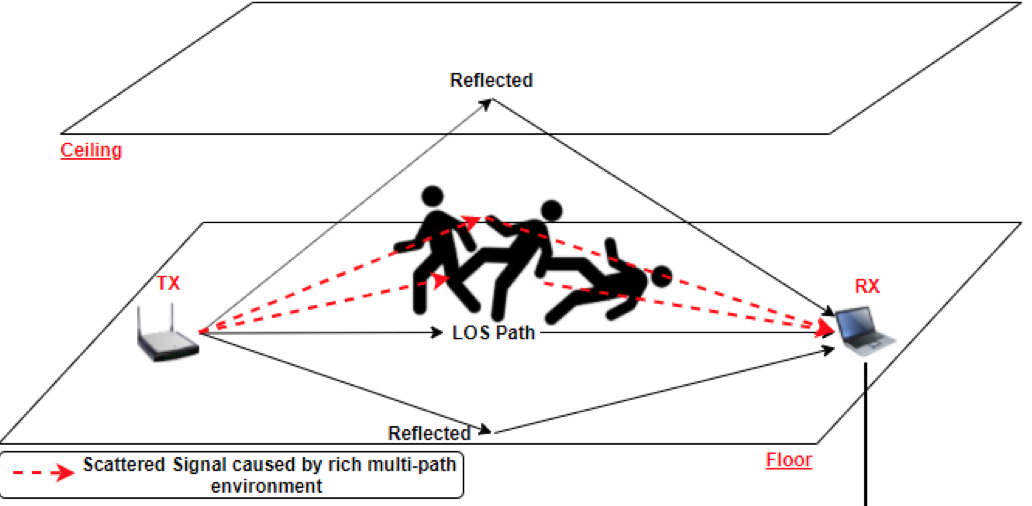
\includegraphics[scale=0.75]{Figures/Reflection.png}
\end{center}
  \caption{The LOS/NLOS paths between the Transmit and Receive antennas in a MIMO system. Note how the scattering environment is created due to the environment structure and the person. Over a short LOS path, small-scale fading characterises the received signal and environment. (Taken from my Interim Presentation)}
  \vspace{-10pt}
  \label{fig:LOS_NLOS}
\end{figure}
A $M\times N$ MIMO system can be modelled by the following equation at the receive antenna by a spatial vector \textbf{y} with a sampling period of T = 1/Bandwidth:
\vspace{-11pt}
\begin{equation}\label{eqn:2.1}
    \textbf{y}(t) = \textbf{H}(t)\textbf{x}(t)+\textbf{n}(t)
    \vspace{-11pt}
\end{equation}
where  $\textbf{x}(t) = \begin{bsmallmatrix}x_1(t) & \cdots & x_M(t)\end{bsmallmatrix}^T$ is the vector of transmitted signals, $\textbf{n}(t) = \begin{bsmallmatrix}n_1(t) & \cdots & n_N(t)\end{bsmallmatrix}^T$ is the AWGN (noise) vector and as mentioned before, $\textbf{H}(t)$ is the channel response matrix for the MIMO system at each time instance $t$ \citep{channelEquations}. \par
The majority of today's Wi-Fi networks operate in the $2-5GHz$ range and thus suffer from the propagation losses mentioned on Page 4. Orthogonal Frequency Division Multiplexing (OFDM) was proposed to offer a robust solution at these frequencies to narrow-band interference. OFDM is the method of digital modulation whereby the signal to be transmitted is split into a number of narrow-band channels at frequencies above and below the centre frequency ($5GHz$ for example) \citep{OFDM}.
These narrow-band channels at different frequencies are also known as \textit{subcarriers} and the method to obtain higher data rates is MIMO-OFDM \citep{802.11nStandard}. OFDM uses a number of modulation schemes such as QAM and PSK. For each OFDM symbol, there are a number of QAM values depending on the channel bandwidth. The application of the IFFT modulates the OFDM symbol onto a number of subcarriers. This is followed by adding cyclic prefix to make the signal robust to multipath propagation \citep{OFDM, 802.11nStandard}. \par
\begin{comment}In Equation \ref{eqn:2.1}, the channel model for a MIMO system is described for a $M\times N$ system.\end{comment}
In a MIMO-OFDM 802.11n system the number of subcarriers is dependent on the bandwidth and group constant. The grouping constant is used to group adjacent subcarriers and report them as a single value to reduce the size of the report field \citep{full802.11nStandard}. Thus, Equation \ref{eqn:2.1} can be rewritten as the following for the subcarrier $k$ at one time instance for a MIMO-OFDM system:
\vspace{-11pt}
\begin{equation}\label{eqn:2.2}
    \textbf{y}_k = \textbf{H}_k\textbf{x}_k+\textbf{n}_k
    \vspace{-11pt}
\end{equation}
where $\textbf{x}_k = \begin{bsmallmatrix}x_{k,1} & \cdots & x_{k,M}\end{bsmallmatrix}^T$ is the transmitted signal vector, $\textbf{n}_k = \begin{bsmallmatrix}n_{k,1} & \cdots & n_{k,N}\end{bsmallmatrix}^T$ is is the noise vector. However, the channel matrix $\textbf{H}_{k}$ can be used to describe the channel response for each transmitter-receiver pair: 
\vspace{-11pt}
\begin{equation}\label{eqn:2.3}
\textbf{h}_{k}=\left[
\begin{array}{ccc}
    h_{k,11} & \cdots & h_{k,M1} \\
   \vdots & \ddots & \vdots \\
    h_{k,1N} & \cdots & h_{k,MN}
\end{array}
\right]
\vspace{-11pt}
\end{equation}
\begin{comment}As there are many subcarriers, there are many of these matrices $\textbf{h}_{k}$.\end{comment}
As described by the 802.11n standard, there are 56 subcarriers for $20MHz$ bandwidth and 114 for $40MHz$ bandwidth with a grouping constant $N_g = 1$.  \citep{full802.11nStandard}.

\textbf{Diagram of MIMO network and also subcarriers around the centre frequency}

\subsection{Channel State Information (CSI)}
The Channel State Information (CSI) describes the Channel Matrix \textbf{H} and thus, the wireless MIMO-OFDM channel itself. It can be described in 3-D matrix form for one packet with \textit{M} transmit antennas, \textit{N} receive antennas for a transmitter-receiver pair(Tx antenna $i$ and Rx antenna $j$)

\textbf{Diagram of the CSI matrix}

The depth of the 3-D matrix as shown above is dependent on the number of subcarriers. Each subcarrier $k$ for a Tx-Rx pair ($ij$) conveys the amplitude/gain and the phase response of the channel at that time instance, $h_{k,ij} = |h_{k,ij}|e^{j\theta}$ \citep{OFDM}. Any change in the channel introduced by either path loss or multi-path fading (See Figure \ref{fig:LOS_NLOS}) will result in Channel Distortion (Amplitude distortion and phase shift).\par 
%%%%%%%%%%%%%%%%%%%%%%%%%%%%%%%%%%%%%%%%%%%%%%%%%%%
COTS Wi-Fi devices do not collect CSI data readily available for the user. With the arrival of the 802.11n WLAN Standard in 2009, transmit beamforming was able to be utilised to estimate the channel over which a beamformee (Rx) and beamformer (Tx) are communicating. It estimates the channel through 2 methods: Implicit feedback and Explicit feedback. In implicit feedback the beamformer receives long trained symbols from the beamformee which it uses to estimate the channel. In explicit feedback, the beamformee makes a direct estimate from the training symbols sent by the beamformer \citep{full802.11nStandard}.The goal is to focus energy towards the receiver to increase the SNR of the wireless channel \citep{beamforming}. The beamformer can maximise the signal power at the receiver depending on the current state of the channel. In a LOS scenario, it is the Tx forming a beam to the Rx directly. \citep{beamforming}. This can give great insight into the changing environment between Tx and Rx. \par
Currently, only Intel and Atheros Wi-Fi NICs can return CSI data through open source tools developed by a number of groups \citep{Halperin_csitool} (Intel NICs) \& \citep{Xie:2015:PPD:2789168.2790124} (Atheros NICs). The CSI of every subcarrier in a MIMO-OFDM Wireless channel is presented as a complex number $a+bj$. The CSI matrix will be of the dimensions $M\times N\times 56$ for a $20MHz$ bandwidth and $M\times N\times 114$ for $40MHz$ bandwidth in theory. In practice, a Wi-Fi NIC uses several bits to represent $a$ \& $b$ (10 bits for each in Atheros NIC and 8 bits in an Intel NIC) \citep{Xie:2015:PPD:2789168.2790124}. This allows the channel to be represented in a number of complex number at a range of subcarrier frequencies. Due to transmit beamforming, we can obtain an accurate model of the channel and the environment. This makes it extremely useful for fall detection, activity detection and indoor localisation where there is a fixed distance between transmitter and receiver. The scattering multi-path environment introduced by an individual will be reported by each data packet's CSI matrix and thus, we can classify the activity. This will be useful for my project for when an individual enters a room, falls, creating a large multi-path scattering environment which will be seen in the CSI data (See Figure \ref{fig:LOS_NLOS}).
%%%%%%%%%%%%%%%%%%%%%%%%%%%%%%%%%%%%%%%%%%%%%%%%%%%%%%%%%%%%%%%%%%%%%%%%%%%%
\begin{comment}\textbf{Can talk about RSSI in the related work section. Some of these do not return in base units so they use the tool which returns in absolute units with AGC added which is da da da da . Talk about how it has been used in indoor localisation, gesture recognition and others and could be used in the thing of all detection as make reference to my diagram because it scatters and suffers from multipath fading and path loss and this will be shown in CSI data at the end corresponding to a movement and then Machine learning can be used for other things}
\end{comment}
%%%%%%%%%%%%%%%%%%%%%%%%%%%%%%%%%%%%%%%%%%%%%%%%%%%%%%%%%%%%%%%%%%%%%
\begin{comment}\subsection{Obtaining CSI information}
As I will be using the Intel Wi-Fi link 5300 Wireless NIC, the open source Linux CSI tool, \cite{Halperin_csitool}, is relevant. It works on an older versions of Ubuntu using customised versions of Intel's close-source firmware and the open-source \textit{iwlwifi} wireless driver \citep{Halperin_csitool}. 
They have also developed user-space measurement tools, access point functionality for both transmitter and receiver and MATLAB scripts for data analysis and pre-processing \citep{Halperin_csitool}. 
There is not enough code space on the NIC for both beamforming software paths and encryption software paths which means CSI data can only be retrieved from non-encrypted access points. 
The CSI data is passed to the kernel driver of the receiver computer which passes the CSI to the user-space program for processing.
In total, 30 groups of sub-carriers evenly across the channel bandwidth are obtained by the Linux tool. Frequency selective fading is clearly seen in the CSI where deeply faded subcarriers due to the environment require the transmitter to expend more power. The tool returns all of the CSI data in a data structure which can be interpreted in MATLAB using provided scripts \citep{Halperin_csitool}.
For example, $get\_scaled\_csi()$ returns the CSI data structure in absolute units rather than Intel's reference level \citep{Halperin_csitool}. \end{comment}
%%%%%%%%%%%%%%%%%%%%%%%%%%%%%%%%%%%%%%%%%%%%%%%%%%%%%%%%%%%%%%%%%%%%%
\section{Related Work \& Existing Fall Detection Systems}
This section deals with current work in the area of CSI and device-free location/activity detection and a literary investigation of the future steps of my project. 
\subsection{CSI and Human detection}
Using the CSI tool, \cite{Halperin_csitool}, it is clear to see there are many applications of CSI data for a wireless channel. The majority of these were carried out by research groups in the areas of indoor localisation \citep{FilaIndoor}, gesture/gait recognition \citep{gestureCSI,GaitRecogCSI}and human activity detection \citep{eEyesActivity}. As mentioned in Chapter \ref{chapter:Introduction}, various wearable approaches have been investigated such as using smartphones for fall detection \citep{smartPhoneFall}. These solutions have obvious disadvantages in terms of needing the device on your person at all times with a suitable level of battery charge. People in most cases either forget to wear them or don't want to. They can be very accurate when all sensors are worn but these may hinder a person's quality of life \citep{ElderlyWearable}. \par
%Look at RSSI and papers in that that came from RT-Fall
As mentioned in Section 2.1, CSI can tell us a lot about the characteristics of the environment. There are a number of attributes in the CSI data across 30 subcarriers which can tell us something about the environment such as the rate of change of the CSI amplitude for the same subcarrier across packets. These attributes can be linked to human activities through a series of supervised learning algorithms in training. The attributes of the CSI data could be matched with a \textit{fall} or \textit{no-fall} activity. Of course, there will be areas where there are fall-like activities such as a person sitting down. This can lead to accurate classification of the activities. 
\begin{comment}From here, a simple binary classifier can be developed having been trained using the supervised Machine Learning algorithm and the attributes of the CSI data. These attributes are typically known as features for the feature extraction stage of the ML algorithm development. This simple classifier will build a model from the training data whereby new, unseen CSI data (test data) can be classified and the performance of the classifier can be determined in terms of True Positive and True Negative classifications. \end{comment}
Clearly using CSI is a useful method for determining human activities in an environment as Wi-Fi access points are readily available around us in today's world. 
\subsection{Fall Detection using CSI}
There are a number of research groups that have completed work in this field such as one of the first systems, WiFall \citep{WiFall}. They achieved 90\% and 94\% fall detection accuracy with different classifiers. As a result, this project is a useful reference. \par
The WiFall system consists of three parts: sensing, learning \& alerting. The sensing phase is the simple transmission of signals from transmitter to receiver. The learning phase is comprised of data processing, profile construction and an activity decision module. The alerting phase triggers an alarm when a fall is detected \citep{WiFall}. As in Section 2.1, the CSI packet is received as a $N_{tx}\times N_{rx}\times 30$ matrix where there a number of transmitter-receiver pairs which WiFall calls \textit{streams}. To simplify the calculations, each stream of 30 values is averaged into one single CSI value for each stream. To do this, they take the CSI value across the full frequency range of subcarriers as in \cite{FilaIndoor}. However, they found that this led to a lack of frequency diversity among CSI subcarriers especially for rich, multi-path environments. As a result, they implemented a moving average filter at each time instance $t$. They have only used the amplitude for activity/anomaly detection and fall detection at $5GHz$ and not the phase. \par
RT-Fall \cite{RTFall}, improves on the methods of WiFall by utilising the phase difference between antennas in a MIMO-OFDM system. They claim that WiFall can only detect falls for four types of predefined activities of walking, sitting, standing up and falling. With WiFall, these activities cannot be performed continuously either \citep{RTFall}. They proposed to use the phase difference over 2 antennas at $5GHz$ as a more sensitive indicator for activity segmentation and fall detection. They find that human activities affect different subcarriers in a similar way and adjacent subcarriers behave similarly. The variance of phase difference across 2 antennas is the sum of the variance on each antenna which implies the phase difference is more sensitive to environment changes than the CSI amplitude making it a more suitable indicator of a fall \citep{PhaseU}. They also discover a sharp power profile decline pattern of a fall in the time-frequency domain. Using these findings, they can segment human activities shown in the CSI data (See Section 2.2.3). They achieve a 14\% higher sensitivity and 10\% higher specificity on average than WiFall \citep{RTFall}.
\subsection{Activity Segmentation}
Taking the CSI data and segmenting it based on different human activities taking place in the environment is crucial. There are many different methods to this such as the one implemented by CARM \citep{CARM}. They used two models to determine a human activity from CSI data: CSI-\textit{speed model} and a CSI-\textit{activity model}. The speed model quantifies the correlation of CSI value dynamics with human movement speeds. The activity model quantifies the movement speeds of different human body parts and a human activity. These 2 models build a correlation between CSI data and the specific activity classifying it appropriately. This ties in with the activity segmentation aspect of my project prior to classification. \par
One of the key steps in activity segmentation is \textit{feature extraction}. In RT-Fall, they use the state transition of the CSI phase difference variance along with the sharp power profile decline pattern to determine the stationary activities and then to further determine fall from fall-like activities \citep{RTFall}. They also found that interpolation is needed in the pre-processing of data. For other pre-processing, they have followed PhaseU and WiFall. As a wireless channel is a shared channel, the devices use random access to share the channel. The received packets are not evenly spaced in the time domain as the transmitter and receiver make no attempt to synchronise timing before transmitting. As the samples are not continuous or evenly spaced in the time domain, Time Frequency analysis for feature extraction cannot take place. To solve this, they follow \cite{gestureCSI} in performing a 1-D linear interpolation algorithm on the raw CSI data. This is followed by band-pass filtering to clean the CSI data of noise and irrelevant frequency components such as breathing or slight movement occurs in the range of [0,4]$Hz$ \citep{RTFall}. To separate fall and fall-like activities, they determine a proper trace back window size for a falling activity. 
\subsection{Feature Extraction \& Classification }
The first step to reliable classification is feature extraction. In \cite{RTFall}, they use the first six features found by \cite{WiFall} and add the \textit{TimeLag} and \textit{Power Decline Ratio} as their own. \textit{TimeLag} is the time delay of the state transition point of an activity between the band-pass filtered and the raw CSI phase difference. In WiFall \citep{WiFall}, they only used the CSI amplitude to extract their six features while in RT-Fall, they extract the first six features from \textit{both the CSI amplitude and phase difference} and extract the last two mentioned features from \textit{CSI phase difference only}. \par
WiFall uses two classifiers, a one-class Support Vector Machine (SVM) and the Random Forest Decision Tree classifier \citep{WiFall}. RT-Fall uses a newer type of SVM classifier called a \textit{v}-SVM classifier \citep{newSVM}. There needs to be an \textit{objective} class (falling) and a \textit{non-objective class} (other activities) which you want to classify correctly and train the model using training (segmented \& labelled) data. In WiFall, falling belongs to the objective class while other human movement belongs to the non-objective class. In RT-Fall, most non-fall like human movements have been removed and the segmentation methods were performed on the fall and fall-like activities. In this case, falling belongs to the objective class and fall-like movements (e.g.,standing up) belong in the non-objective class \citep{WiFall,RTFall}. With user feedback, the classifier model can be tuned by re-labelling incorrect classifications and updating the model. Both WiFall and RT-Fall have used LibSVM to develop their classification models \citep{LibSVM}. \par
Other CSI fall detection projects have used SVMs \citep{antiFall}, k-NN(Nearest Neighbour) algorithms \citep{robustdevicefree}, Decision Trees \citep{WiFall,Dayal2016HumanFD} and Neural Networks \citep{Dayal2016HumanFD}. For example, Decision trees are useful because they do not assume any inherent relationship between each of the features while SVMs with a Gaussian Kernel assume a Gaussian distribution of the feature vector. \citep{Dayal2016HumanFD}. For rich multi-path environments with many classes, one-class SVMs are not suitable and perform poorly where Decision Trees do well. \par
